\documentclass[tikz,border=2pt]{standalone}
\usepackage{amsmath}
\usetikzlibrary{arrows.meta}
\begin{document}
% SVD of A = [[3,0],[4,5]] as three steps, all drawn to one scale (k = 0.45 cm per unit):
% V^T sends v_1, v_2 to e_1, e_2; Sigma stretches them by sigma_1 = 3 sqrt5, sigma_2 = sqrt5;
% U turns them into sigma_1 u_1 = A v_1 = (3,9)/sqrt2 and sigma_2 u_2 = A v_2 = (3,-1)/sqrt2.
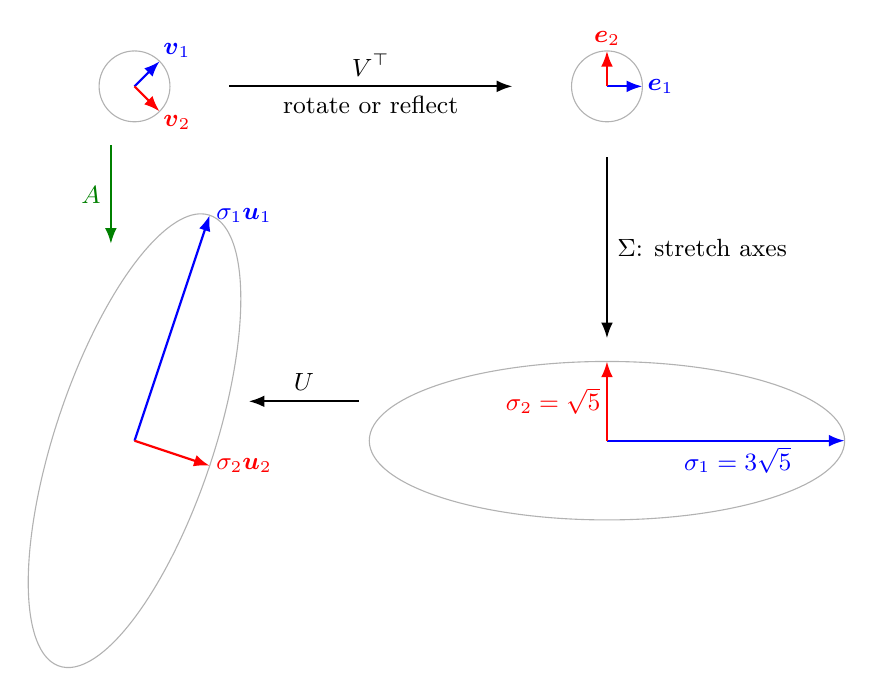
\begin{tikzpicture}[font=\small, >={Latex[length=2mm]}]
  \def\k{0.45}
  % top left: unit circle with right singular vectors
  \begin{scope}[shift={(0,0)}]
    \draw[gray!60] (0,0) circle (\k);
    \draw[->, thick, blue] (0,0) -- ({\k*0.7071},{\k*0.7071}) node[above right, inner sep=1pt] {$\boldsymbol{v}_1$};
    \draw[->, thick, red] (0,0) -- ({\k*0.7071},{-\k*0.7071}) node[below right, inner sep=1pt] {$\boldsymbol{v}_2$};
  \end{scope}
  % top right: after V^T
  \begin{scope}[shift={(6,0)}]
    \draw[gray!60] (0,0) circle (\k);
    \draw[->, thick, blue] (0,0) -- (\k,0) node[right, inner sep=1.5pt] {$\boldsymbol{e}_1$};
    \draw[->, thick, red] (0,0) -- (0,\k) node[above, inner sep=1.5pt] {$\boldsymbol{e}_2$};
  \end{scope}
  % bottom right: after Sigma
  \begin{scope}[shift={(6,-4.5)}]
    \draw[gray!60] (0,0) ellipse ({\k*6.7082} and {\k*2.2361});
    \draw[->, thick, blue] (0,0) -- ({\k*6.7082},0) node[pos=0.55, below, inner sep=2pt] {$\sigma_1=3\sqrt{5}$};
    \draw[->, thick, red] (0,0) -- (0,{\k*2.2361}) node[pos=0.5, left, inner sep=2pt] {$\sigma_2=\sqrt{5}$};
  \end{scope}
  % bottom left: after U, the image A(unit circle)
  \begin{scope}[shift={(0,-4.5)}]
    \draw[gray!60] plot[domain=0:360, samples=120, smooth] ({\k*3*cos(\x)},{\k*(4*cos(\x)+5*sin(\x))});
    \draw[->, thick, blue] (0,0) -- ({\k*2.1213},{\k*6.3640}) node[right, inner sep=2pt] {$\sigma_1\boldsymbol{u}_1$};
    \draw[->, thick, red] (0,0) -- ({\k*2.1213},{-\k*0.7071}) node[right, inner sep=2pt] {$\sigma_2\boldsymbol{u}_2$};
  \end{scope}
  % the three steps and the composite map
  \draw[->, thick] (1.2,0) -- (4.8,0) node[midway, above] {$V^{\top}$} node[midway, below] {rotate or reflect};
  \draw[->, thick] (6,-0.9) -- (6,-3.2) node[midway, right] {$\Sigma$: stretch axes};
  \draw[->, thick] (2.85,-4.0) -- (1.45,-4.0) node[midway, above] {$U$};
  \draw[->, thick, green!50!black] (-0.3,-0.75) -- (-0.3,-2.0) node[midway, left] {$A$};
\end{tikzpicture}
\end{document}
